\documentclass[class=article, crop=false]{standalone}
\usepackage[subpreambles=true]{standalone}
\usepackage{import}
\usepackage[T1]{fontenc}
\usepackage[utf8]{inputenc}
\usepackage[english, danish]{babel}
\usepackage{graphicx,wrapfig,lipsum}

\begin{document}

    \begin{figure}[H]
        \centering

        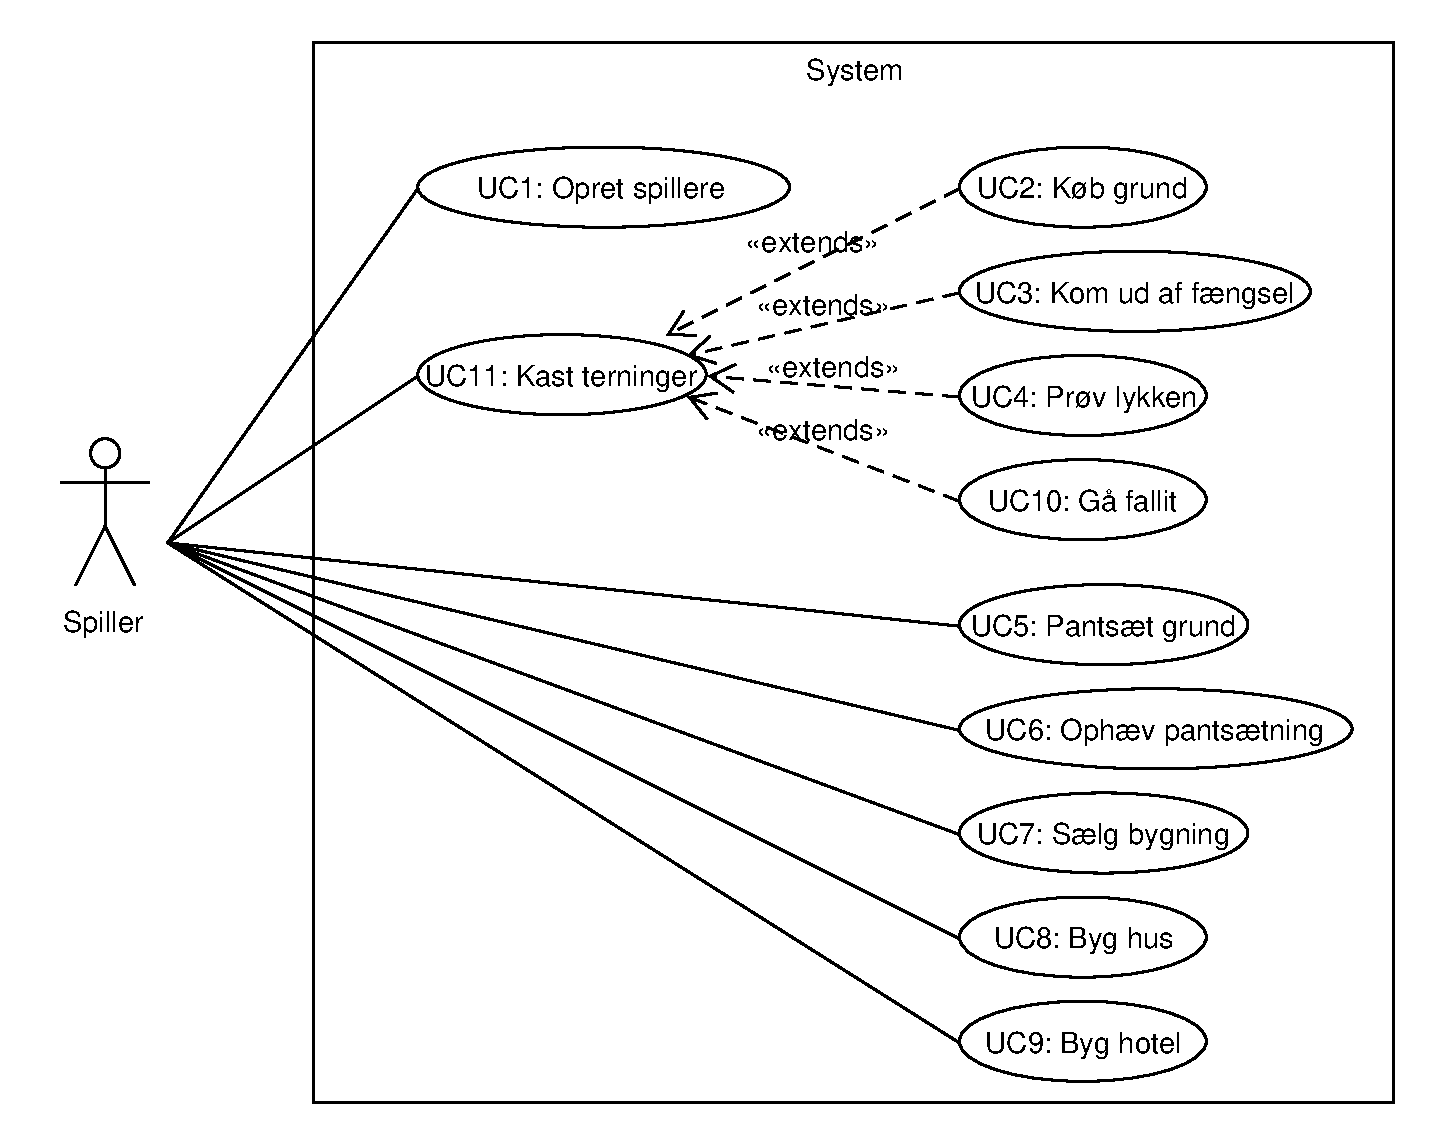
\includegraphics[scale=0.7]{diagrams/use_case_diagram.pdf}
        \caption{Use case diagram over systemet}\label{fig:use_case_model}
    \end{figure}

    Ovenstående use-case diagram på Figur~\ref{fig:use_case_model} viser de forskellige use cases relationer til spilleren, samt deres indbyrdes sammenhæng. Det kan ses, at det blev besluttet at opdele, hvad der kunne have været en use case (som nok ville kaldes, “Spil spillet”) op i flere use cases, for bedre overblik over programmets forskellige elementer.

\end{document}